
% This LaTeX was auto-generated from MATLAB code.
% To make changes, update the MATLAB code and republish this document.

\documentclass{article}
\usepackage{graphicx}
\usepackage{color}

\sloppy
\definecolor{lightgray}{gray}{0.5}
\setlength{\parindent}{0pt}

\begin{document}

    
    
\subsection*{Contents}

\begin{itemize}
\setlength{\itemsep}{-1ex}
   \item Problem 7.43
   \item Set up RVs
   \item Plots
\end{itemize}


\subsection*{Problem 7.43}

\begin{verbatim}
clear; close all; clc;
\end{verbatim}


\subsection*{Set up RVs}

\begin{verbatim}
N=1000000; % Set number of samples
z=[0:0.1:20]; % define variable for horizontal axis
w=randn(3,N).*4 + 3; % generate uniform random samples
W = sqrt(w(1,:).^2 + w(2,:).^2 + w(3,:).^2);
F=zeros(1,length(z)); % initialize CDF estimate
for n=1:N % estimate CDF
F=F+(W(n)<z);
end
F=F/N;
\end{verbatim}


\subsection*{Plots}

\begin{par}
CDF
\end{par} \vspace{1em}
\begin{verbatim}
figure(1)
plot(z,F) % plot results
xlabel('x'); ylabel('F_X(x)')

% PDF
figure(2)
fx = diff(F);
plot(z(1:end-1),fx)
xlabel('x'); ylabel('f_X(x)')
\end{verbatim}

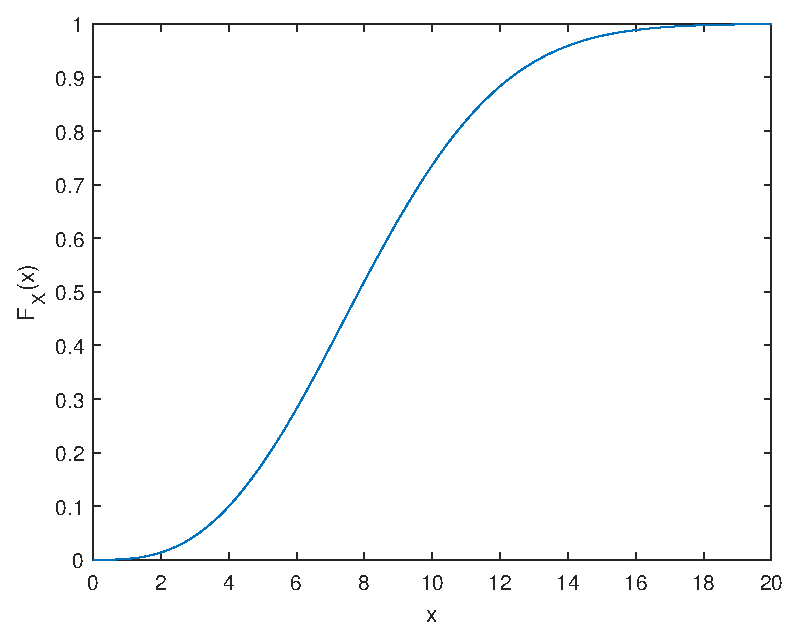
\includegraphics [width=4in]{prob7_43_01.eps}

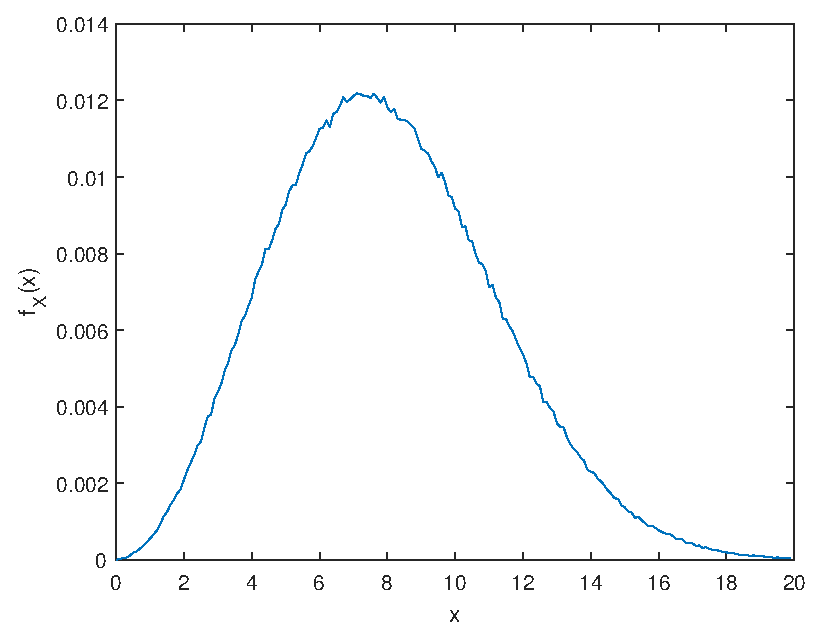
\includegraphics [width=4in]{prob7_43_02.eps}



\end{document}
    
